\shortdescription{In this activity we practice evaluating functions at
  numbers and other functions.} 
\activitytitle{Evaluating Functions}


\begin{theorem}[Hello]
\end{theorem}

\begin{proof}[solution] Obvious!\link{http:lkjflkdjf}
\end{proof}


\begin{exercise}
Given that $f(x)=-5 x^4+2 x^3+x^2-3 x+2$, evaluate $f(3.9)$.\video{hello}
\begin{solution}
\begin{hint}
$f(3.9)=-5 (3.9)^4+2 (3.9)^3+(3.9)^2-3 (3.9)+2$.
\end{hint}
\begin{hint}
$f(3.9)=-1032.57$.
\end{hint}
The value of the function $f(x) = -5 x^4+2 x^3+x^2-3 x+2$, evaluated at $x=3.9$, is $\answer{-1032.57}$.
\end{solution}
\end{exercise}


\begin{question}
\begin{multiple-choice}
\choice[correct]{Hello!}
\choice{NO!}
\end{multiple-choice}
\begin{solution}
\begin{hint}
Hello is always right!
\end{hint}
\end{solution}
\end{question}





\begin{question}
In the plot below, is $B$ a function of $z$?
\begin{image}
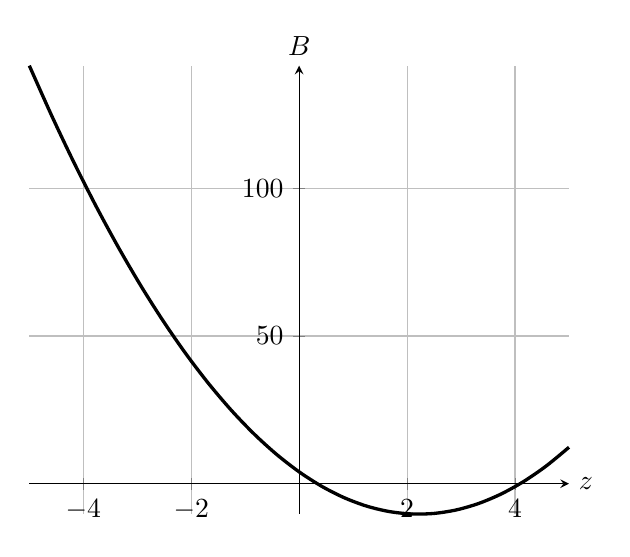
\begin{tikzpicture}
\begin{axis}[
            clip=false,
            axis lines =center, xlabel=$z$, ylabel=$B$,
              every axis y label/.style={at=(current axis.above origin),anchor=south},
              every axis x label/.style={at=(current axis.right of origin),anchor=west},
            domain=-5:5,
            grid = major,
          ]
          \addplot [very thick, smooth] {4 + (-5/4 + (35*(-4 + x))/12)*x};
        \end{axis}
\end{tikzpicture}
\end{image}
\begin{multiple-choice}
\choice[correct]{Yes.}
\choice{No.}
\end{multiple-choice}
\begin{solution}
\begin{hint}
For each input, how many outputs are there?
\end{hint}
\end{solution}
Use the plot to compute $B(0)$
\begin{solution}
\begin{hint}
To start, find $0$ on the horizontal axis. 
\end{hint}
\begin{hint}
Now from this position, move up or down until you reach the curve. The value of $B(0)$ is the height of the curve at the point $z=0$.
\end{hint}
The value of $B(0)$ is \answer{$4$}.
\end{solution}
Is $B^{-1}$ a function of $z$ on the domain $[-10,141]$?
\begin{multiple-choice}
\choice{Yes.}
\choice[correct]{No.}
\end{multiple-choice}
\begin{solution}
\begin{hint}
For each input of $B^{-1}$, how many outputs are there?
\end{hint}
\end{solution}
Restrict the domain of $B$ to $[3,5]$ and compute $B^{-1}(4)$.
\begin{solution}
\begin{hint}
Since we are looking at $B^{-1}$, now we must find $-1$ on the vertical axis. 
\end{hint}
The value of $B^{-1}(-1)$ is \answer{$4$}.
\end{solution}
\end{question}



\begin{question}
In the plot below, is $B$ a function of $z$?
\begin{figure}[h]
\begin{center}
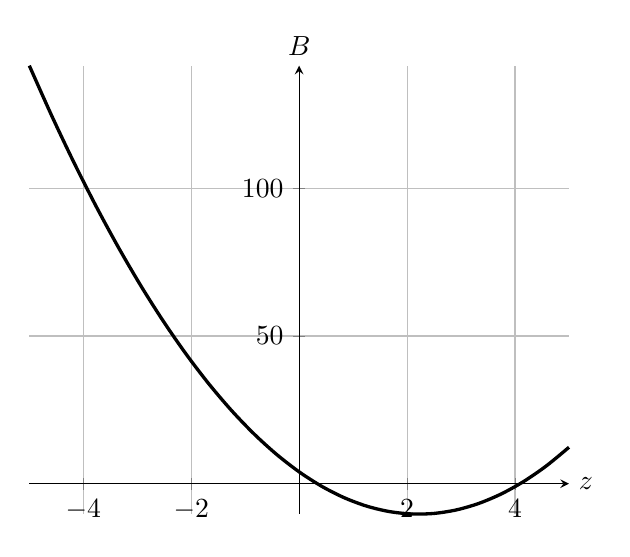
\begin{tikzpicture}
\begin{axis}[
            clip=false,
            axis lines =center, xlabel=$z$, ylabel=$B$,
              every axis y label/.style={at=(current axis.above origin),anchor=south},
              every axis x label/.style={at=(current axis.right of origin),anchor=west},
            domain=-5:5,
            grid = major,
          ]
          \addplot [very thick, smooth] {4 + (-5/4 + (35*(-4 + x))/12)*x};
        \end{axis}
\end{tikzpicture}
\end{center}
\end{figure}
\begin{multiple-choice}
\choice[correct]{Yes.}
\choice{No.}
\end{multiple-choice}
\begin{solution}
\begin{hint}
For each input, how many outputs are there?
\end{hint}
\end{solution}
Use the plot to compute $B(0)$
\begin{solution}
\begin{hint}
To start, find $0$ on the horizontal axis. 
\end{hint}
\begin{hint}
Now from this position, move up or down until you reach the curve. The value of $B(0)$ is the height of the curve at the point $z=0$.
\end{hint}
The value of $B(0)$ is \answer{$4$}.
\end{solution}
Is $B^{-1}$ a function of $z$ on the domain $[-10,141]$?
\begin{multiple-choice}
\choice{Yes.}
\choice[correct]{No.}
\end{multiple-choice}
\begin{solution}
\begin{hint}
For each input of $B^{-1}$, how many outputs are there?
\end{hint}
\end{solution}
Restrict the domain of $B$ to $[3,5]$ and compute $B^{-1}(4)$.
\begin{solution}
\begin{hint}
Since we are looking at $B^{-1}$, now we must find $-1$ on the vertical axis. 
\end{hint}
The value of $B^{-1}(-1)$ is \answer{$4$}.
\end{solution}
\end{question}
